\chapter{Attaque SSLStrip}

\label{sec:sslstrip}

\begin{figure}[H]
  \caption{Attaque SSLStrip (diagramme Dia)}
  \fbox{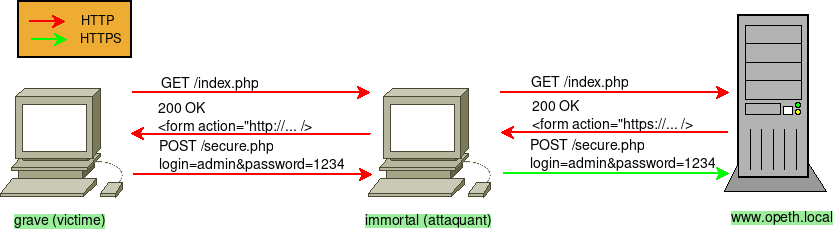
\includegraphics[width=\textwidth]{../medias/sslstrip/attack.png}}
\end{figure}

\section{Description de l'attaque}

L'attaque SSLStrip a été présentée pour la première fois en 2009 par l'américain Moxie Marlinspike à la conférence de sécurité Blackhat. C'est une attaque très simple qui va permettre à un attaquant de pouvoir récupérer des informations confidentielles telles qu'un mot de passe ou un cookie de session. Cependant, l'attaque n'est plus vraiment d'actualité, nous reviendrons là dessus à la fin.

Pour que l'attaquant puisse utiliser SSLStrip, il doit pouvoir se placer en homme du milieu entre le client et le serveur. C'est à dire qu'il doit être capable d'intercepter le trafic entre ces deux derniers, et pouvoir le modifier à sa guise. Bien sûr, l'attaquant n'a aucun intérêt à substituer une requête du client pour envoyer n'importe quoi à la place, car le serveur ne comprendra pas la requête et fermera la connexion TCP. Il va donc falloir être astucieux dans la manière dont on agit.

Pour pouvoir se placer en homme du milieu, il y a plusieurs façons de procéder. Une des façons les plus simples consiste à se placer dans le réseau privé de la victime, et de faire de l'ARP spoofing/poisonning. L'idée étant de faire croire au routeur qu'il parle à la victime, et vice versa, en falsifiant leurs tables ARP respectives (cette table donnant la correspondance entre adresse MAC et adresse IP). L'attaquant va ainsi pouvoir lire tout le trafic qui circule entre la victime et le routeur (donc entre la victime et le serveur).

Une fois placé en homme du milieu, l'attaquant peut donc voir et intercepter le trafic envoyé par la victime vers le serveur. Bien sûr, si ce trafic est chiffré, par exemple avec le protocole SSL/TLS, alors l'attaquant ne pourra rien en tirer, à moins de trouver une faille dans le chiffrement utilisé. Ici, on ne va pas essayer de casser TLS, mais plus de profiter du fait que toutes les requêtes envoyées par le client ne sont pas chiffrées (ce qui est de moins en moins le cas de nos jours).

Ainsi, si la requête du client est une simple requête HTTP, l'attaquant va pouvoir lire en clair ce qu'il envoie, et mieux encore, il va également voir la réponse du serveur.

On sait donc maintenant que notre attaquant peut, si la requête n'est pas chiffrée, lire l'échange effectué entre le client et le serveur, et même le modifier un peu si la requête reste valide et compréhensible par le serveur. Mais, que va-t-on bien pouvoir modifier pour obtenir des informations intéressantes ?

Pour répondre à cette question, il faut savoir que toutes les pages sensibles d'un site internet (qui demandent une connexion avec identifiant/mot de passe), ne sont accessibles que par une requête sécurisée en HTTPS (ou alors le site est vraiment peu précautionneux). Lorsqu'une page HTML contient des liens vers des pages sécurisées, ces liens sont donc en HTTPS, pour indiquer au client qu'un chiffrement va être nécessaire à la connexion d'une page en particulier.

\begin{figure}[H]
  \caption{Exemple d'une page HTML avec un lien sécurisé en HTTPS}
  \fbox{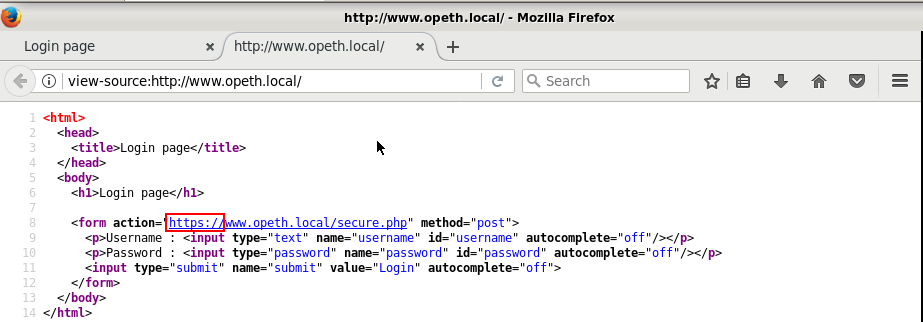
\includegraphics[width=\textwidth]{../medias/sslstrip/screen2.png}}
\end{figure}

L'idée de l'attaque, va donc être de forcer le client à se connecter en HTTP, et non en HTTPS, sur la page sensible. Pour cela, rien de plus simple : lorsque le serveur va envoyer une page HTML contenant des liens HTTPS, l'attaquant va simplement intercepter la page HTML, retirer le 's' de chacun de ces liens, et envoyer la page au client. Lorsque ce dernier voudra se connecter sur ces liens, il le fera donc en HTTP et non en HTTPS comme il l'aurait fallu. L'attaquant va donc pouvoir lire tout le trafic de cette requête HTTP, contenant par exemple un mot de passe si la page sécurisée était un formulaire de connexion.

\begin{figure}[H]
  \caption{La même page HTML, où l'attaquant a retiré le 's'}
  \fbox{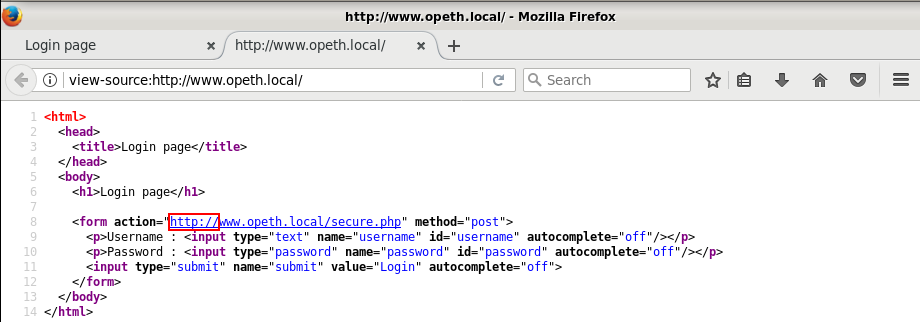
\includegraphics[width=\textwidth]{../medias/sslstrip/screen5.png}}
\end{figure}

Les actions à mettre en place pour réaliser l'attaque sont les suivantes :

\begin{enumerate}
\item Regarder le trafic HTTP
\item Changer les liens HTTPS par des HTTP et garder en mémoire cette conversion
\item Lorsque le client fait HTTP pour une URL qui devrait être en HTTPS, il faut envoyer au serveur la même requête en HTTPS
\item Conserver une carte des liens relatifs, CSS, JavaScript
\item Pour essayer de conserver le même aspect visuel, on doit faire de même pour les favicon en renvoyant la favicon de notre choix
\item A éliminer des en-têtes de requêtes, les encodages, les cookies et les pages en cache.
\item Lors des requêtes POST envoyées par SSL, avec login et password, il faut faire expirer les cookies pour que l'utilisateur renvoie une requête sans cookies
\end{enumerate}

\section{Notre attaque}

\subsection{Mise en place de l'environnement}

Pour cette attaque, nous utilisons un seul domaine : \path{www.opeth.local}. Nous avons alors deux pages, \path{index.php} et \path{secure.php}, la première étant accédée en HTTP et la seconde en HTTPS.

Pour la résolution des noms de domaines, nous utilisons les fichiers \path{/etc/hosts} des différentes machines.

\subsection{Démonstration}

Pour lancer l'attaque, nous utilisons l'outil qemunet comme ceci :

\begin{minted}{bash}
./qemunet/qemunet.sh -x -S sslstrip
\end{minted}

À partir de là, les trois machines sont lancées.

\subsubsection{Étape 1 : avant l'attaque}

Lorsque l'attaque n'est pas encore lancée, nous pouvons voir sur la machine grave, que tout se passe normalement et que la requête POST passe bien en HTTPS (immortal est donc incapable de voir les identifiants envoyés) :

\begin{figure}[H]
  \caption{Attaque SSLStrip (avant l'attaque)}
  \fbox{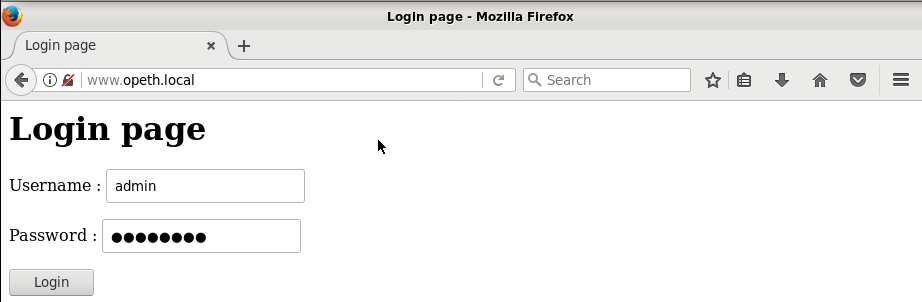
\includegraphics[width=\textwidth]{../medias/sslstrip/screen1.png}}
\end{figure}

L'encadré rouge suivant montre bien que le POST est effectué en HTTPS, sur la page secure.php.

\begin{figure}[H]
  \caption{Code source de la page (avant l'attaque)}
  \fbox{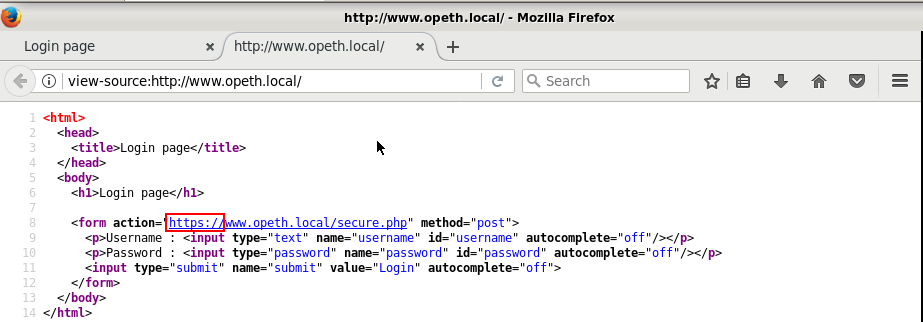
\includegraphics[width=\textwidth]{../medias/sslstrip/screen2.png}}
\end{figure}

Nous arrivons alors sur la page \path{secure.php}, en HTTPS : la machine immortal n'a pas pût voir nos échanges sur cette page sécurisée.

\begin{figure}[H]
  \caption{Code source de la page (avant l'attaque)}
  \fbox{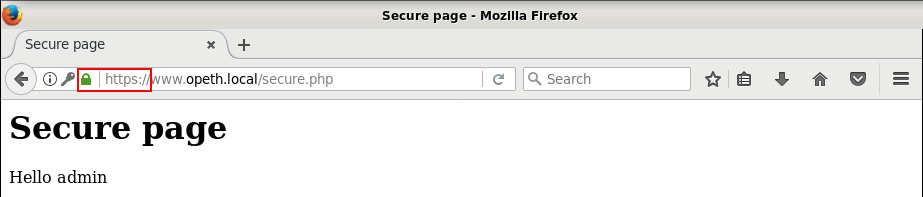
\includegraphics[width=\textwidth]{../medias/sslstrip/screen3.png}}
\end{figure}

\subsubsection{Étape 2 : lancement de l'attaque}

Comme expliqué précédemment, pour lancer l'attaque, il faut exécuter le fichier \path{/mnt/host/attack.sh} depuis immortal. Voici son contenu :

\begin{minted}{bash}
PROXY_PORT=4242

iptables -t nat -F
iptables -t nat -A PREROUTING -p tcp --destination-port 80 -j REDIRECT --to-port $PROXY_PORT

/mnt/host/sslstrip.py $PROXY_PORT
\end{minted}

La règle iptables permet de rediriger les flux TCP à destination du port 80 (HTTP) vers le port d'écoute du proxy qui est chargé d'analyser et traiter les requêtes.

\begin{figure}[H]
  \caption{Lancement de l'attaque}
  \fbox{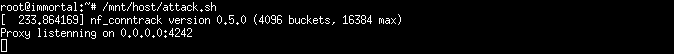
\includegraphics[width=\textwidth]{../medias/sslstrip/screen4.png}}
\end{figure}

\paragraph{Explication du code du proxy \\}

Le code du proxy est dans le fichier \path{sslstrip.py}.

\subparagraph{Réception des requêtes \\}

Lors de la réception de requêtes, il s'agit de savoir si l'on doit :

\begin{itemize}
\item fermer la connexion (le client ou le serveur a fermé sa socket)
\item établir une connexion HTTPS, dans le cas où le client demande la page secure.php
\item établir une connexion HTTP, dans le cas où le client demande la page d'accueil index.php
\end{itemize}

Voici la fonction implémentant la réception d'une requête HTTP :

\begin{minted}{python}
def __recv(self, csock):
        fw_sock = self.__csockets[csock]
        data = csock.recv(BUFFER_SIZE)
        if len(data) == 0:
            self.__close_conn(csock)
            self.__close_conn(fw_sock)
        else:
            print(data)

            if fw_sock is None:
                m = re.search(b'(GET|POST) (\S+) HTTP/\d.\d', data)
                if m is not None and m.group(2) in HTTPS_URL:
                    self.__new_https_conn(csock)
                else:
                    self.__new_http_conn(csock)
                fw_sock = self.__csockets[csock]
            data = self.__replace_https_to_http(data)
            data = self.__replace_content_length(data)
            fw_sock.send(data)
\end{minted}

A la fin, on transforme tous les liens https trouvé en http et on recalcule la taille de la requête (entête Content-Length).

\subparagraph{Transformation des liens \\}

La transformation se fait à l'aide d'une expression régulière qui remplace \path{https://} par \path{http://} dans les données HTTP.

\begin{minted}{python}
def __replace_https_to_http(self, data):
        return re.sub(b'https://', b'http://', data)
\end{minted}

\subparagraph{Recalcule de l'entête Content-Length \\}

Il faut ensuite recalculer l'entête Content-Length, en se basant sur le début des données HTTP situées après la séquence "{\textbackslash}r{\textbackslash}n{\textbackslash}r{\textbackslash}n" :

\begin{minted}{python}
def __replace_content_length(self, data):
    try:
        idx = data.index(b"\r\n\r\n")
        length = len(data) - idx - 4
        return re.sub(b'Content-Length: (\d+)',
                      b'Content-Length: %d' % length, data, 1)
    except:
        return data
\end{minted}

\subsubsection{Étape 3 : pendant l'attaque}

Lorsque l'attaque est lancée, on peut voir que tous les liens \path{https://} sont remplacés par \path{http://}.

La machine immortal est donc capable d'intercepter les échanges réalisés sur la page secure.php. Ici on voit dans l'encadré rouge, que le lien \path{https://} a bien été remplacé par un lien non sécurisé \path{http://} :

\begin{figure}[H]
  \caption{Le 's' de "https" a disparu}
  \fbox{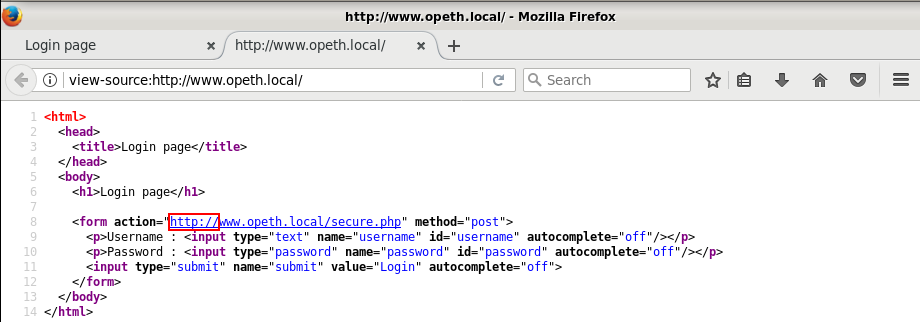
\includegraphics[width=\textwidth]{../medias/sslstrip/screen5.png}}
\end{figure}

Nous constatons que nous arrivons sur la page secure.php en HTTP : notre navigation n'est pas sécurisée !

\begin{figure}[H]
  \caption{Le client visite une page sécurisée en http}
  \fbox{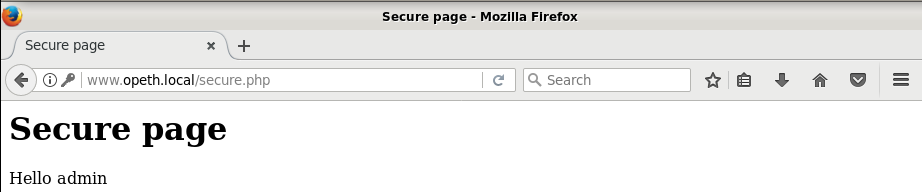
\includegraphics[width=\textwidth]{../medias/sslstrip/screen6.png}}
\end{figure}

La machine immortal a été capable de capturer non seulement les identifiants du formulaire, mais également le cookie de session :

\begin{figure}[H]
  \caption{L'attaquant récupère toutes les informations sensibles}
  \fbox{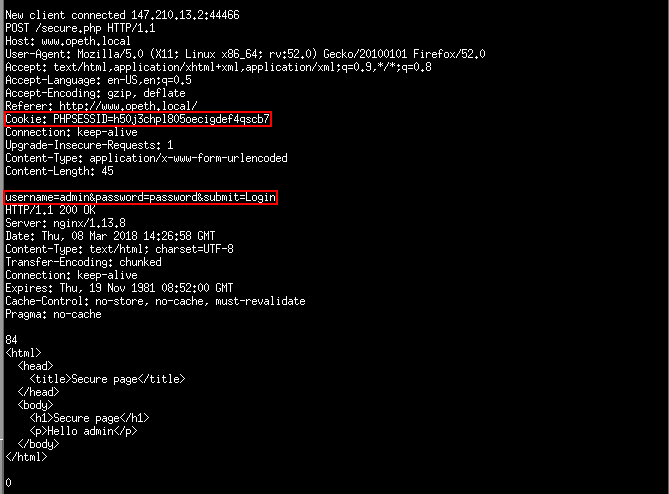
\includegraphics[width=\textwidth]{../medias/sslstrip/screen7.png}}
\end{figure}

Le script complet de l'attaque peut être consulté à l'annexe \ref{appendix:sslstrip}.

\section{Limitations de notre attaque}

Cependant, l'attaque n'est plus vraiment d'actualité car les sites internet modernes (ou plutôt, ceux qui pensent à la sécurité de leurs utilisateurs), utilisent HTTPS sur toutes les pages de leur site web, ce qui empêche l'attaquant d'intercepter ne serait-ce qu'une requête HTTP, et de la modifier. De plus, une autre protection, nommée HSTS, permet au serveur d'indiquer à un client de toujours se connecter en HTTPS sur certaines pages. Ainsi, si un attaquant parvient à intercepter une requête HTTP, et à remplacer les liens HTTPS vers des liens HTTP dans le code HTML, le navigateur du client émettra une exception, car il aura gardé en mémoire qu'il doit se connecter en HTTPS sur telle page spécifique. Néanmoins il existe des moyens de contourner cet ajout, nous en parlerons dans la prochaine attaque.

Notre implémentation est volontairement minimaliste, et nous ne traitons pas certains détails. Par exemple, les redirections (code HTTP 3XX) n'ont pas été réellement prisent en compte par notre script, mais peuvent être également attaquées. Aussi, notre outil s'occupe simplement de rediriger les requêtes vers un domaine fixé à l'avance. Un vrai programme mémoriserait les différentes requêtes en redirigeant vers le bon domaine à chaque fois.
